\documentclass[11pt,spanish,a4paper]{article}
% Versión 1.er cuat 2021 Víctor Bettachini < bettachini@df.uba.ar >

% Versión 1.er cuat 2021 Víctor Bettachini < bettachini@df.uba.ar >

\usepackage[T1]{fontenc}
\usepackage[utf8]{inputenc}

\usepackage[spanish, es-tabla]{babel}
\def\spanishoptions{argentina} % Was macht dass?
% \usepackage{babelbib}
% \selectbiblanguage{spanish}
% \addto\shorthandsspanish{\spanishdeactivate{~<>}}

\usepackage{graphicx}
\graphicspath{{./figuras/}}
% \usepackage{float}

\usepackage[arrowdel]{physics}
\newcommand{\pvec}[1]{\vec{#1}\mkern2mu\vphantom{#1}}
% \usepackage{units}
\usepackage[separate-uncertainty=true, multi-part-units=single, locale=FR]{siunitx}
\usepackage{isotope} % $\isotope[A][Z]{X}\to\isotope[A-4][Z-2]{Y}+\isotope[4][2]{\alpha}

\usepackage{tasks}
\usepackage[inline]{enumitem}
% \usepackage{enumerate}

\usepackage{hyperref}

% \usepackage{amsmath}
% \usepackage{amstext}
\usepackage{amssymb}

\usepackage{tikz}
\usepackage{tikz-dimline}
\usetikzlibrary{math}
\usetikzlibrary{arrows.meta}
% \usetikzlibrary{snakes}
% \usetikzlibrary{calc}
\usetikzlibrary{decorations.pathmorphing}
\usetikzlibrary{patterns}

\usepackage[hmargin=1cm,vmargin=1.6cm,nohead]{geometry}
% \voffset-3.5cm
% \hoffset-3cm
% \setlength{\textwidth}{17.5cm}
% \setlength{\textheight}{27cm}

\usepackage{lastpage}
\usepackage{fancyhdr}
\pagestyle{fancyplain}
\fancyhead{}
\fancyfoot{{\tiny \textcopyright DF, FCEyN, UBA}}
\fancyfoot[C]{ {\tiny Actualizado al \today} }
\fancyfoot[RO, LE]{Pág. \thepage/\pageref{LastPage}}
\renewcommand{\headrulewidth}{0pt}
\renewcommand{\footrulewidth}{0pt}


\begin{document}
\begin{center}
	\textbf{Física 2} (Físicos) \hfill \textcopyright {\tt DF, FCEyN, UBA}\\
	\textsc{\LARGE Difracción}
\end{center}

Los ejercicios con (*) entrañan una dificultad adicional. Son para investigar después de resolver los demás.


\begin{enumerate}

\section*{Difracción de Fraunhofer}

\item
\begin{enumerate}
	\item Considere la figura de difracción de Fraunhofer producida por una rendija de ancho $b$ ubicada entre dos lentes convergentes y centrada en el eje óptico del sistema.
La fuente puntual de longitud de onda $\lambda$ se coloca en el foco de la primera lente. 
	\begin{enumerate}
		\item ¿Dónde se coloca la pantalla de observación?
		\item Calcule la posición de los máximos y de los mínimos de irradiancia, el ancho angular de la campana principal de difracción y de los máximos secundarios. 
		\item Calcule la relación de irradianciaes entre el máximo principal y el primer máximo secundario. 
		\item Grafique la irradiancia sobre la pantalla.
		¿En función de qué variables lo hace?
		¿Podría haber elegido otras?, ¿cuáles?
		\item Discuta cómo se modifican los parámetros de la figura de difracción si se cambia: 1) el ancho de la ranura, 2) la longitud de onda, 3) si se coloca una fuente policromática. 
	\end{enumerate}
	\item Idem a), si la fuente se encuentra en el plano focal de la primera lente, a una altura $h$ del eje óptico. 
	\item Idem b), si la ranura se centra a una altura $h'$ del eje óptico. 
\end{enumerate}



\item Una rendija de \SI{50}{\micro\metre} de ancho se encuentra entre dos lentes delgadas convergentes de igual distancia focal, y está iluminada por ondas planas, de longitud de onda $\lambda = \SI{5000}{\angstrom}$.
La distancia entre el primer mínimo a la izquierda del máximo principal y el tercer mínimo a su derecha es de \SI{3}{\milli\metre}.
Además, el primer mínimo a la izquierda está ubicado \SI{3}{\milli\metre} a la derecha del eje óptico.
\begin{enumerate}
	\item ¿Cuál es la distancia focal de las lentes? 
	\item ¿Dónde se encuentra la fuente?
	¿Dónde el máximo principal? 
\end{enumerate}



\item La distancia entre el primer y el quinto mínimos de un patrón de difracción producido por una sola rendija es de \SI{0.35}{\centi\metre}.
La pantalla sobre la cual se despliega el patrón está a \SI{40}{\centi\metre} de la abertura y la longitud de onda es de \SI{550}{\nano\metre}.
¿Cuál es el ancho de la rendija?



\item Una rendija se ilumina con luz cuyas longitudes de onda \(\lambda_1\) y \(\lambda_2\) se escogen de tal manera que el primer mínimo de difracción de \(\lambda_1\) coincida con el segundo mínimo de \(\lambda_2\).
\begin{enumerate}
	\item ¿Qué relación existe entre las dos longitudes de onda?
	\item ¿Coinciden algunos otros mínimos en los dos patrones de difracción?
\end{enumerate}



\subsection*{Patrón de difracción bidimensional}

\item
\begin{enumerate}
	\item (*) Hallar el patrón de irradianciaes de una abertura rectangular de lados $a$ y $b$, que se encuentra a distancia $D$ de una pantalla.
	Considere incidencia normal. 
	\item (*) Idem para una abertura circular de radio $a$.
\end{enumerate}



\item (*)
\begin{minipage}[t][2.5cm]{0.6\textwidth}
Hallar el campo eléctrico, como función de las coordenadas sobre la pantalla, para las configuraciones de la figura, las que se encuentran a distancia $D$ de la pantalla.
La luz es monocromática de longitud de onda $\lambda$ e incide normalmente sobre las aberturas. 
\end{minipage}
\begin{minipage}[c][2.5cm][t]{0.3\textwidth}
	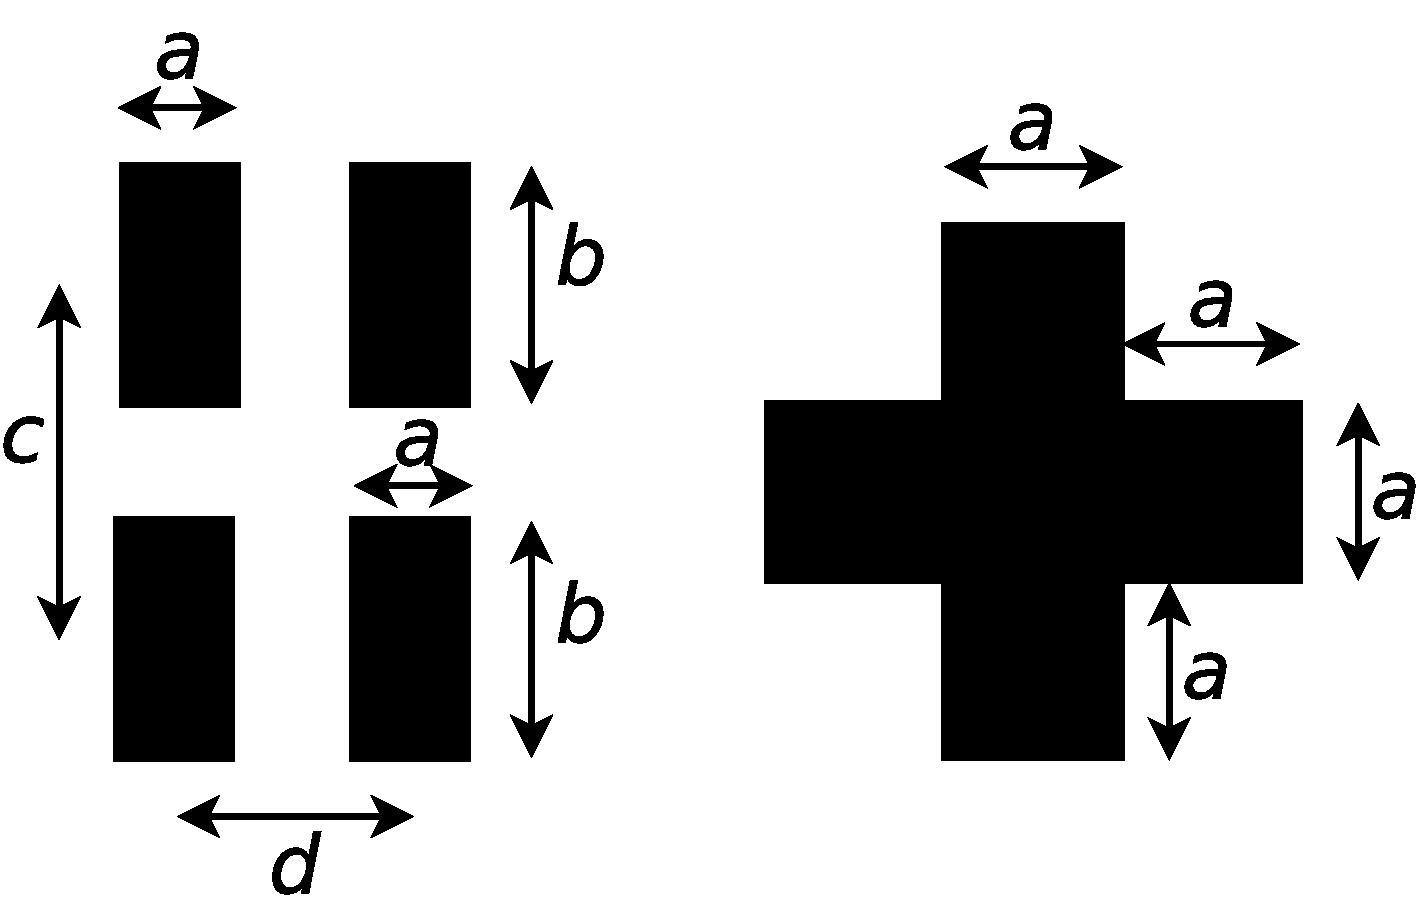
\includegraphics[width=\textwidth]{ej5-35}
\end{minipage}

\section*{Límite de resolución por difracción}

\item Sean dos fuentes puntuales incoherentes colocadas en el plano focal objeto de una lente convergente; ambas emiten la misma $\lambda$.
A la derecha de la lente hay una ranura de ancho $b$, y luego una segunda lente.
Se observa la figura de difracción de Fraunhofer de las fuentes.
\begin{enumerate}
	\item Calcule la mínima separación angular entre las fuentes, y la correspondiente mínima separación lineal, para que las imágenes estén justamente resueltas según el criterio de Rayleigh.
	Discuta los casos en que ambas fuentes emiten con la misma irradiancia, y en que no. 
	\item Repita el cálculo efectuado en a) si la rendija se reemplaza por una abertura circular de diámetro $d$.
\end{enumerate}



\item Suponga al ojo humano limitado por difracción, y calcule el mínimo ángulo que resuelve para un diámetro de pupila de \SI{2}{\milli\metre}.
Si dos puntos se hallan a la distancia de visión clara, ¿cuál es la mínima distancia entre ellos para que estén justamente resueltos?



\end{enumerate}

\end{document}
